\section{Rendering pipeline}
\label{sec:chapter_stato_arte_rendering_pipeline}

Il processo di generazione di immagini 2D dato un insieme di oggetti 3D, delle fonti di luce e delle texture, si decompone in una successione di passi di elaborazione; tale successione è detta pipeline di rendering. 
Nella visione più elementare di questa pipeline è possibile individuare tre fasi: \emph{Applicazione}, \emph{Geometria} e \emph{Rasterizzazione}.
Ognuna di queste fasi è essa stessa una pipeline i cui passi possono essere parallelizzati, o anch’essi messi in pipeline. La velocità complessiva del processo viene determinata dal passo più lento della pipeline, ed è espressa in immagini renderizzate per secondo (FPS).

A differenza delle vecchie pipeline di rendering, dove tutto il processo viene eseguito sulla CPU, l’odierna fruibilità di un hardware dedicato all’accelerazione grafica consente di spostare su di esso l’esecuzione di alcuni passi. Infatti, mentre lo stadio Applicazione è sviluppato interamente in software ed eseguito sulla CPU, gli stadi Geometria e Rasterizzazione sono eseguiti sull’unita di processamento grafico (GPU).
\\
\begin{figure}[htb]
 \centering
 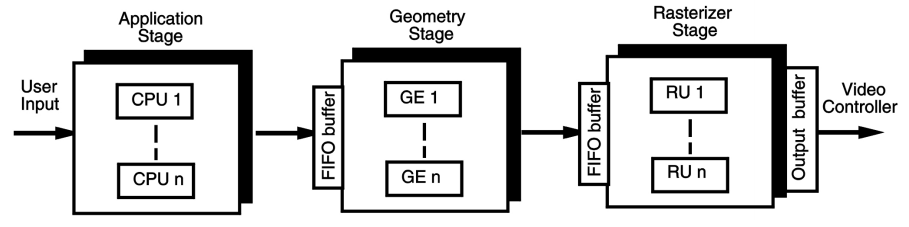
\includegraphics[width=1.0\linewidth]{images/chapter_stato_arte/stato_arte_pipeline.png}\hfill
 \caption[Pipeline di rendering]{Pipeline di rendering}
 \label{fig:stato_arte_pipeline}
\end{figure}

Il livello applicazione è quello più flessibile; infatti lo sviluppatore ne ha pieno controllo e ne può modificare l’implementazione. I cambiamenti effettuati su questo livello possono incidere sulle performance dei livelli successivi. 
Questa prima fase ha due compiti fondamentali: gestire gli input che possono provenire da più sorgenti, come tastiera o mouse, ed inviare allo step successivo la posizione della camera, le informazioni sulle luci presenti nella scena e le primitive di rendering.
Quest’ ultime rappresentano la descrizione in punti, spigoli e triangoli, delle entità geometriche presenti nella scena e sono il dato di input fondamentale per gli hardware grafici. 
Come esempio pratico si può fare riferimento all’editor mostrato più avanti in questo elaborato: tale strumento consente di selezionare e muovere oggetti o parti di esso. 
In questo caso il livello Applicazione si occupa di tradurre il movimento del mouse nella corrispondente matrice di rotazione da applicare all’oggetto che si è scelto di ruotare. 
Inoltre questo livello si occuperà, ad ogni ciclo di rendering, di inviare allo stadio Geometria la posizione della camera, le informazioni sulle luci e le primitive di rendering dei modelli presenti nella scena.

Il livello Geometria è il passo dove vengono effettuate la maggior parte delle operazioni su vertici e triangoli. A differenza del livello Applicazione, questo secondo stadio si può decomporre in una successione di sotto-processi.
Inizialmente ad ogni oggetto della scena è associato un sistema di riferimento in coordinate modello, rispetto al quale l’oggetto appare immobile. 
Per posizionare ed orientare ogni oggetto nello stesso sistema di riferimento è necessario applicare ad ognuno una trasformazione del modello.  Tale trasformazione opererà sui vertici e sulle normali di ogni oggetto per posizionarli nel sistema di riferimento in coordinate mondo, unico per ogni modello, rispetto al quale gli oggetti appariranno posizionati ed orientati in base alle trasformazioni di modello applicate. 
Siccome al processo di renderizzazione partecipano solo gli oggetti che la camera vede, bisogna applicare un’ulteriore trasformazione alla camera e a tutti i modelli della scena. 
Tale trasformazione converte tutti gli oggetti della scena da un sistema di riferimento in coordinate mondo ad uno in coordinate camera. 
In questo nuovo sistema di riferimento la camera è posizionata nell’origine e punta verso le z negative, con l’asse y che punta verso l’alto e l’asse x orientata verso destra.
\\
\begin{figure}[htb]
 \centering
 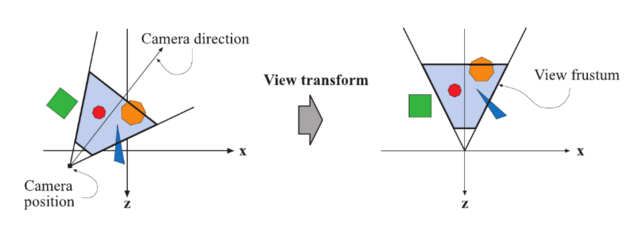
\includegraphics[width=1.0\linewidth]{images/chapter_stato_arte/stato_arte_view_transform.png}\hfill
 \caption[Trasformazione della vista]{In foto è possibile notare la trasformazione di ogni oggetto da un sistema di riferimento in coordinate mondo, ad uno in coordinate della camera.}
 \label{fig:stato_arte_trasfvista}
\end{figure}

Forma e posizione degli oggetti non sono l’unico aspetto chiave per un rendering realistico; infatti anche le informazioni sui materiali di ogni oggetto, così come l’effetto di ogni fonte luminosa nella scena, risultano fondamentali. 
Il processo di determinazione di un effetto luminoso su di una superficie composta da un certo materiale è detta \emph{shading}. 
Tale processo consiste nel calcolo di una equazione di shading in corrispondenza dei vertici dell’oggetto. Ogni vertice può memorizzare diverse informazioni, come la posizione dell’ oggetto, una normale, un colore, o qualsiasi altra informazione necessaria al calcolo dell’equazione, il cui risultato può essere ad esempio un colore, un vettore o una coordinata di una texture. 
E’ importante che il calcolo delle equazioni di shading venga effettuato in un sistema di riferimento comune a tutti gli oggetti, in modo che le relazioni tra oggetti, camera, e luci rimangano preservate. 
Dopo lo shading, il processo di rendering si occupa della trasformazione del volume di vista percepito dalla camera in un cubo unitario detto volume di vista canonico.
Tipicamente vengono usati due metodi di proiezione: ortografica e prospettica (Fig \ref{fig:stato_arte_trasfvista}).
In quella ortografica il volume di vista appare come un parallelepipedo rettagolo, e la proprietà fondamentale è che le linee parallele rimangano tali dopo la trasformazione.
Nella proiezione prospettica invece viene simulato il modo in cui noi percepiamo la dimensione degli oggetti: tanto più un oggetto si allontana dalla camera, tanto più sarà piccolo dopo la proiezione. In questo caso le linee parallele convergono all’orizzonte, e il volume di vista è rappresentato come una piramide tronca con base rettangolare.
Un oggetto che subisce una delle due proiezioni  si dice appartenente al sistema di riferimento con coordinate normalizzate della camera. 
\\
\begin{figure}[htb]
 \centering
 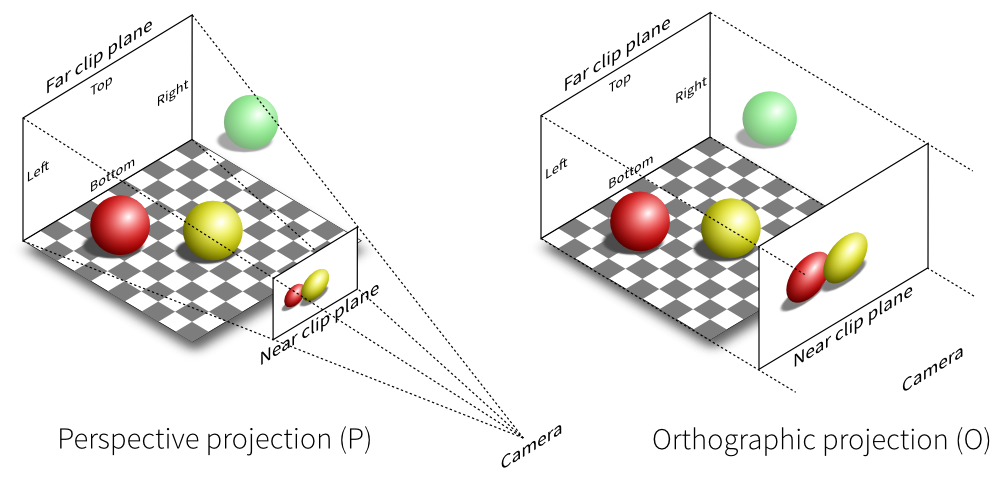
\includegraphics[width=1.0\linewidth]{images/chapter_stato_arte/stato_arte_projections.png}\hfill
 \caption[Proiezione prospettica ed ortogonale]{Volume di vista nella proiezione ortografica (a sinistra), e prospettica (a destra)}
 \label{fig:stato_arte_projections}
\end{figure}

A questo punto, dato un volume di vista, sono note le primitive di rendering da dare in input alla fase di rasterizzazione, dove verrano finalmente disegnate su schermo.
Se una primitiva risiede all’interno del volume passerà allo stadio successivo, così come verrà ignorata se presente al di fuori di esso. 
Per quanto riguarda le primitive che si trovano parzialmente all’interno del volume di vista è necessario un ulteriore passo di elaborazione, detto clipping. 
La trasformazione in coordinate camera, e la proiezione, fanno si che il clipping possa essere effettuato con riferimento ad un volume di vista rappresentato da un cubo unitario.
Si consideri ad esempio uno spigolo con un vertice nel volume di vista e con l’altro fuori; è sufficiente calcolare un nuovo vertice nell’intersezione tra lo spigolo ed il cubo unitario, scartando così il vertice esterno.
\\
\begin{figure}[htb]
 \centering
 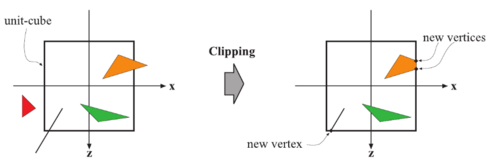
\includegraphics[width=1.0\linewidth]{images/chapter_stato_arte/stato_arte_clipping.png}\hfill
 \caption[Clipping]{Clipping}
 \label{fig:stato_arte_clipping}
\end{figure}

A questo punto le primitive nel volume di vista, le quali sono ancora descritte in coordinate a tre dimensioni, sono passate alla fase di mappatura su schermo. 
Nella mappatura le coordinate x,y di ogni primitiva sono trasformate in coordinate di schermo, mentre la z non subisce alcuna mappatura.
Le coordinate di schermo insieme alla z costituiscono le coordinate di finestra, le quali vengono passate alla fase di rasterizzazione.
\\
\begin{figure}[htb]
 \centering
 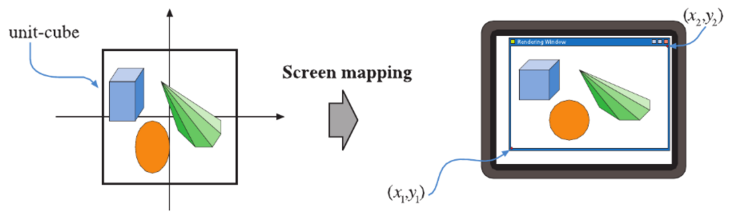
\includegraphics[width=1.0\linewidth]{images/chapter_stato_arte/stato_arte_mapping.png}\hfill
 \caption[Mappatura su schermo]{Mappatura su schermo delle primitive nel volume di vista}
 \label{fig:stato_arte_mapping}
\end{figure}

A questo punto le coordinate di finestra, insieme alle informazioni di shading associate ad ogni vertice, vengono convertite in pixel sullo schermo. Come avvenuto per la  fase Geometria, il processo può essere decomposto in più passi.

Inizialmente vengono computate le informazioni necessarie alla fase successiva; tali informazioni saranno utili, ad esempio, per l’interpolazione dei dati di shading computati nella fase Geometria.
Per ogni pixel vengono individuati dei frammenti, ovvero porzioni di pixel posizionate all’interno di un triangolo. Le proprietà di ogni frammento sono calcolate mediante interpolazione dei dati memorizzati sui vertici del triangolo di cui fa parte. 
Tali proprietà includono:

\begin{itemize}
\item La profondità del frammento: l’interpolazione della coordinata (di finestra) z sui vertici del triangolo di cui il frammento fa parte.
\item I dati di shading calcolati nella fase Geometria.
\end{itemize}

I dati di shading interpolati sono necessari al calcolo dello shading sui frammenti di pixel, il cui risultato è un colore da dare in input alla fase successiva.
In quest’ultima fase del processo di rasterizzazione vengono dapprima memorizzate le informazioni di ogni pixel in un buffer di colori, detto pixel buffer, ovvero un array dove ogni elemento è un pixel con un informazione a 3 componenti di colore: rosso, verde e blu.
A questo punto il colore ottenuto dallo shading sui frammenti di pixel ed il colore memorizzato nel buffer sono combinati.
Tale buffer deve contenere il colore relativo alle primitive di scena visibili dal punto di vista della camera. 
Per individuare quali oggetti sono visibili e quali non lo sono all’interno della scena viene utilizzato un ulteriore buffer, detto \emph{z-buffer}. Questo buffer ha stesse dimensioni e forma del pixel buffer, e per ogni pixel viene memorizzata la distanza tra la camera e la primitiva di rendering più vicina ad essa.
Quando una primitiva deve essere renderizzata su un determinato pixel, il valore z tra la primitiva e il pixel del piano immagine della camera viene confrontato con quello memorizzato nello z buffer:

\begin{itemize}
\item Se il nuovo valore z è più piccolo di quello memorizzato nel buffer, allora la nuova primitiva è più vicina alla camera di quanto lo fosse quella relativa al valore di z memorizzato nel buffer. A questo punto vengono aggiornati z-buffer e pixel buffer, entrambi nella stessa posizione: il primo con il nuovo valore z, il secondo con il colore relativo alla nuova primitiva da renderizzare. 
\item Se invece il nuovo valore z è più grande di quello memorizzato nel buffer, non vi è alcun aggiornamento.
\end{itemize}

\begin{figure}[htb]
 \centering
 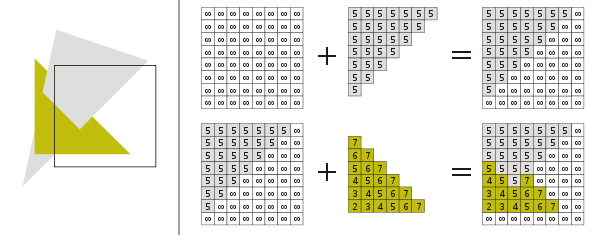
\includegraphics[width=1.0\linewidth]{images/chapter_stato_arte/stato_arte_z_buffer.png}\hfill
 \caption[Z-buffer]{Z-buffer}
 \label{fig:stato_arte_z_buffer}
\end{figure}

Z-buffer è sicuramente un algoritmo molto semplice, e dalla complessità computazionale ridotta; infatti essa cresce linearmente con il numero di primitive da renderizzare (O(n)). Le primitive, nella maggior parte dei casi, sono renderizzabili in qualsiasi ordine. 
Tuttavia ciò non vale per alcune primitive, come quelle trasparenti. In questo caso è necessario impartire un ordinamento: per prima cosa si renderizzano tutte le primitive opache, in ordine qualsiasi, dopodichè si passa a quelle trasparenti, in ordine dalla più distante alla più vicina. 
Se per le primitive trasparenti non fosse seguito questo ordinamento sarebbe impossibile miscelare i colori di più oggetti posizionati uno di fronte all’altro. Questo si rende necessario per via del comportamento dello z-buffer insieme al pixel-buffer.
Quando ad esempio viene osservato un filtro trasparente rosso di fronte ad un oggetto opaco blu, l’ occhio miscela insieme i due colori permettendo di osservare una tonalità magenta nella porzione in cui i due oggetti sono sovrapposti.
Disegnare prima l’oggetto blu, più distante, memorizzandone nei rispettivi z-buffer e pixel-buffer i corrispondenti dati di distanza e colore, permette quando viene disegnato anche il filtro rosso di prelevare queste informazioni dai buffer al fine di miscelare i due colori.
Il colore blu del primo oggetto viene infatti combinato con il rosso del secondo oggetto in base alla trasparenza di quest’ultimo.
\\
\begin{figure}[htb]
 \centering
 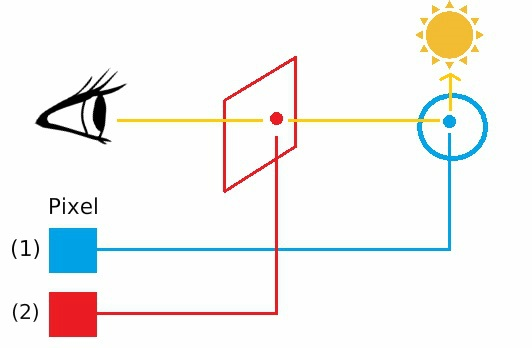
\includegraphics[width=0.8\linewidth]{images/chapter_stato_arte/stato_arte_zbuffer_1.jpg}\hfill
 \caption[Z-buffer: ordine di renderizzazione corretto]{Z-buffer: scenario in cui l'ordine di renderizzazione è dall'oggetto più distante, a quello più vicino}
 \label{fig:stato_arte_zbuffer_1}
\end{figure}
 
Se invece questo ordine fosse invertito e quindi il filtro rosso venisse renderizzato prima dell’oggetto blu, sarebbe impossibile miscelare i due colori.
Questo perchè l’algoritmo di z-buffer considererebbe il secondo oggetto renderizzato, quello blu, nascosto dal filtro rosso in quanto più distante dall’ occhio. Le informazioni dell’ oggetto blu verrebbero quindi scartate perchè inutili, non permettendo così la combinazione dei due colori.
\\
\begin{figure}[htb]
 \centering
 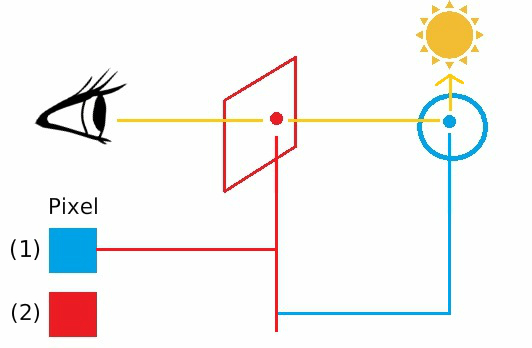
\includegraphics[width=0.8\linewidth]{images/chapter_stato_arte/stato_arte_zbuffer_2.jpg}\hfill
 \caption[Z-buffer: ordine di renderizzazione errato]{Z-buffer: scenario in cui l'ordine di renderizzazione è l'inverso di quello mostrato in figura \ref{fig:stato_arte_zbuffer_1}}
 \label{fig:stato_arte_zbuffer_2}
\end{figure}

Ovviamente le primitive completamente trasparenti non vengono considerate, e per  distinguere tra primitive parzialmente o completamente trasparenti, viene fatto uso di un ulteriore buffer associato al pixel buffer. Tale buffer contiene, per ogni pixel, un valore alpha che indica il grado di opacità relativo al pixel. Se tale valore è uguale ad 1 il pixel risulta completamente opaco. La trasparenza del pixel aumenta al decrementare del valore alpha; per alpha uguale a zero il pixel è completamente trasparente e non viene considerato per le fasi successive.

La fase di rasterizzazione offre inoltre la possibilità di istruire lo z buffer e il pixel buffer su quali primitive renderizzare. Questo è possibile utilizzando un array contenente 8 bit per pixel chiamato \emph{stencil-buffer}. Le primitive che decidiamo di renderizzare nello stencil buffer, corrisponderanno a quelle che dovranno essere renderizzate nello z buffer e nel pixel buffer. Se ad esempio disegnassimo un cerchio all’interno dello stencil buffer, le primitive che verranno renderizzate nello z buffer e nel pixel buffer saranno solamente quelle presenti all’interno del cerchio.

Nel corso degli anni sono stati sviluppati diversi algoritmi di renderizzazione ed ognuno utilizza tecniche differenti per ottenere l’immagine finale. I limiti del rasterization render nel calcolo delle informazioni di luce hanno spinto verso la sperimentazione di tecniche più efficienti nella modellazione degli effetti luminosi all’interno di una scena.